% =============================================================
%  Plan 08 — SFT training pipeline
%  version v0.1 (2026-06-01)
%  Trainer: llm_infra/train.py :: BPTTTrainer
% =============================================================
\documentclass[border=10pt,tikz]{standalone}
\usepackage{tikz}
\usepackage{amsmath,amssymb}
\usetikzlibrary{positioning,fit,shapes.geometric,arrows.meta,calc,backgrounds,
                decorations.pathreplacing}

\definecolor{frozenfill}{HTML}{E8ECEF}
\definecolor{trainedfill}{HTML}{FFE6B3}
\definecolor{datafill}{HTML}{D8E8FB}
\definecolor{lossfill}{HTML}{FDE2E2}
\definecolor{teacherfill}{HTML}{E0EBF6}
\definecolor{gradclr}{HTML}{C0392B}
\definecolor{arrowclr}{HTML}{2B2B2B}

\tikzset{
  block/.style    = {draw, rounded corners=2pt, inner sep=4pt,
                     align=center, font=\small},
  frozen/.style   = {block, fill=frozenfill},
  trained/.style  = {block, fill=trainedfill, very thick},
  data/.style     = {block, fill=datafill},
  loss/.style     = {block, fill=lossfill, very thick,
                     font=\small\bfseries, minimum width=80mm},
  teacher/.style  = {block, fill=teacherfill, dashed},
  flow/.style     = {-Latex, thick, draw=arrowclr},
  align/.style    = {<->, thick, draw=arrowclr!70, dashed, font=\footnotesize},
  grad/.style     = {-Latex, thick, draw=gradclr, dashed, font=\footnotesize\bfseries},
}

\begin{document}
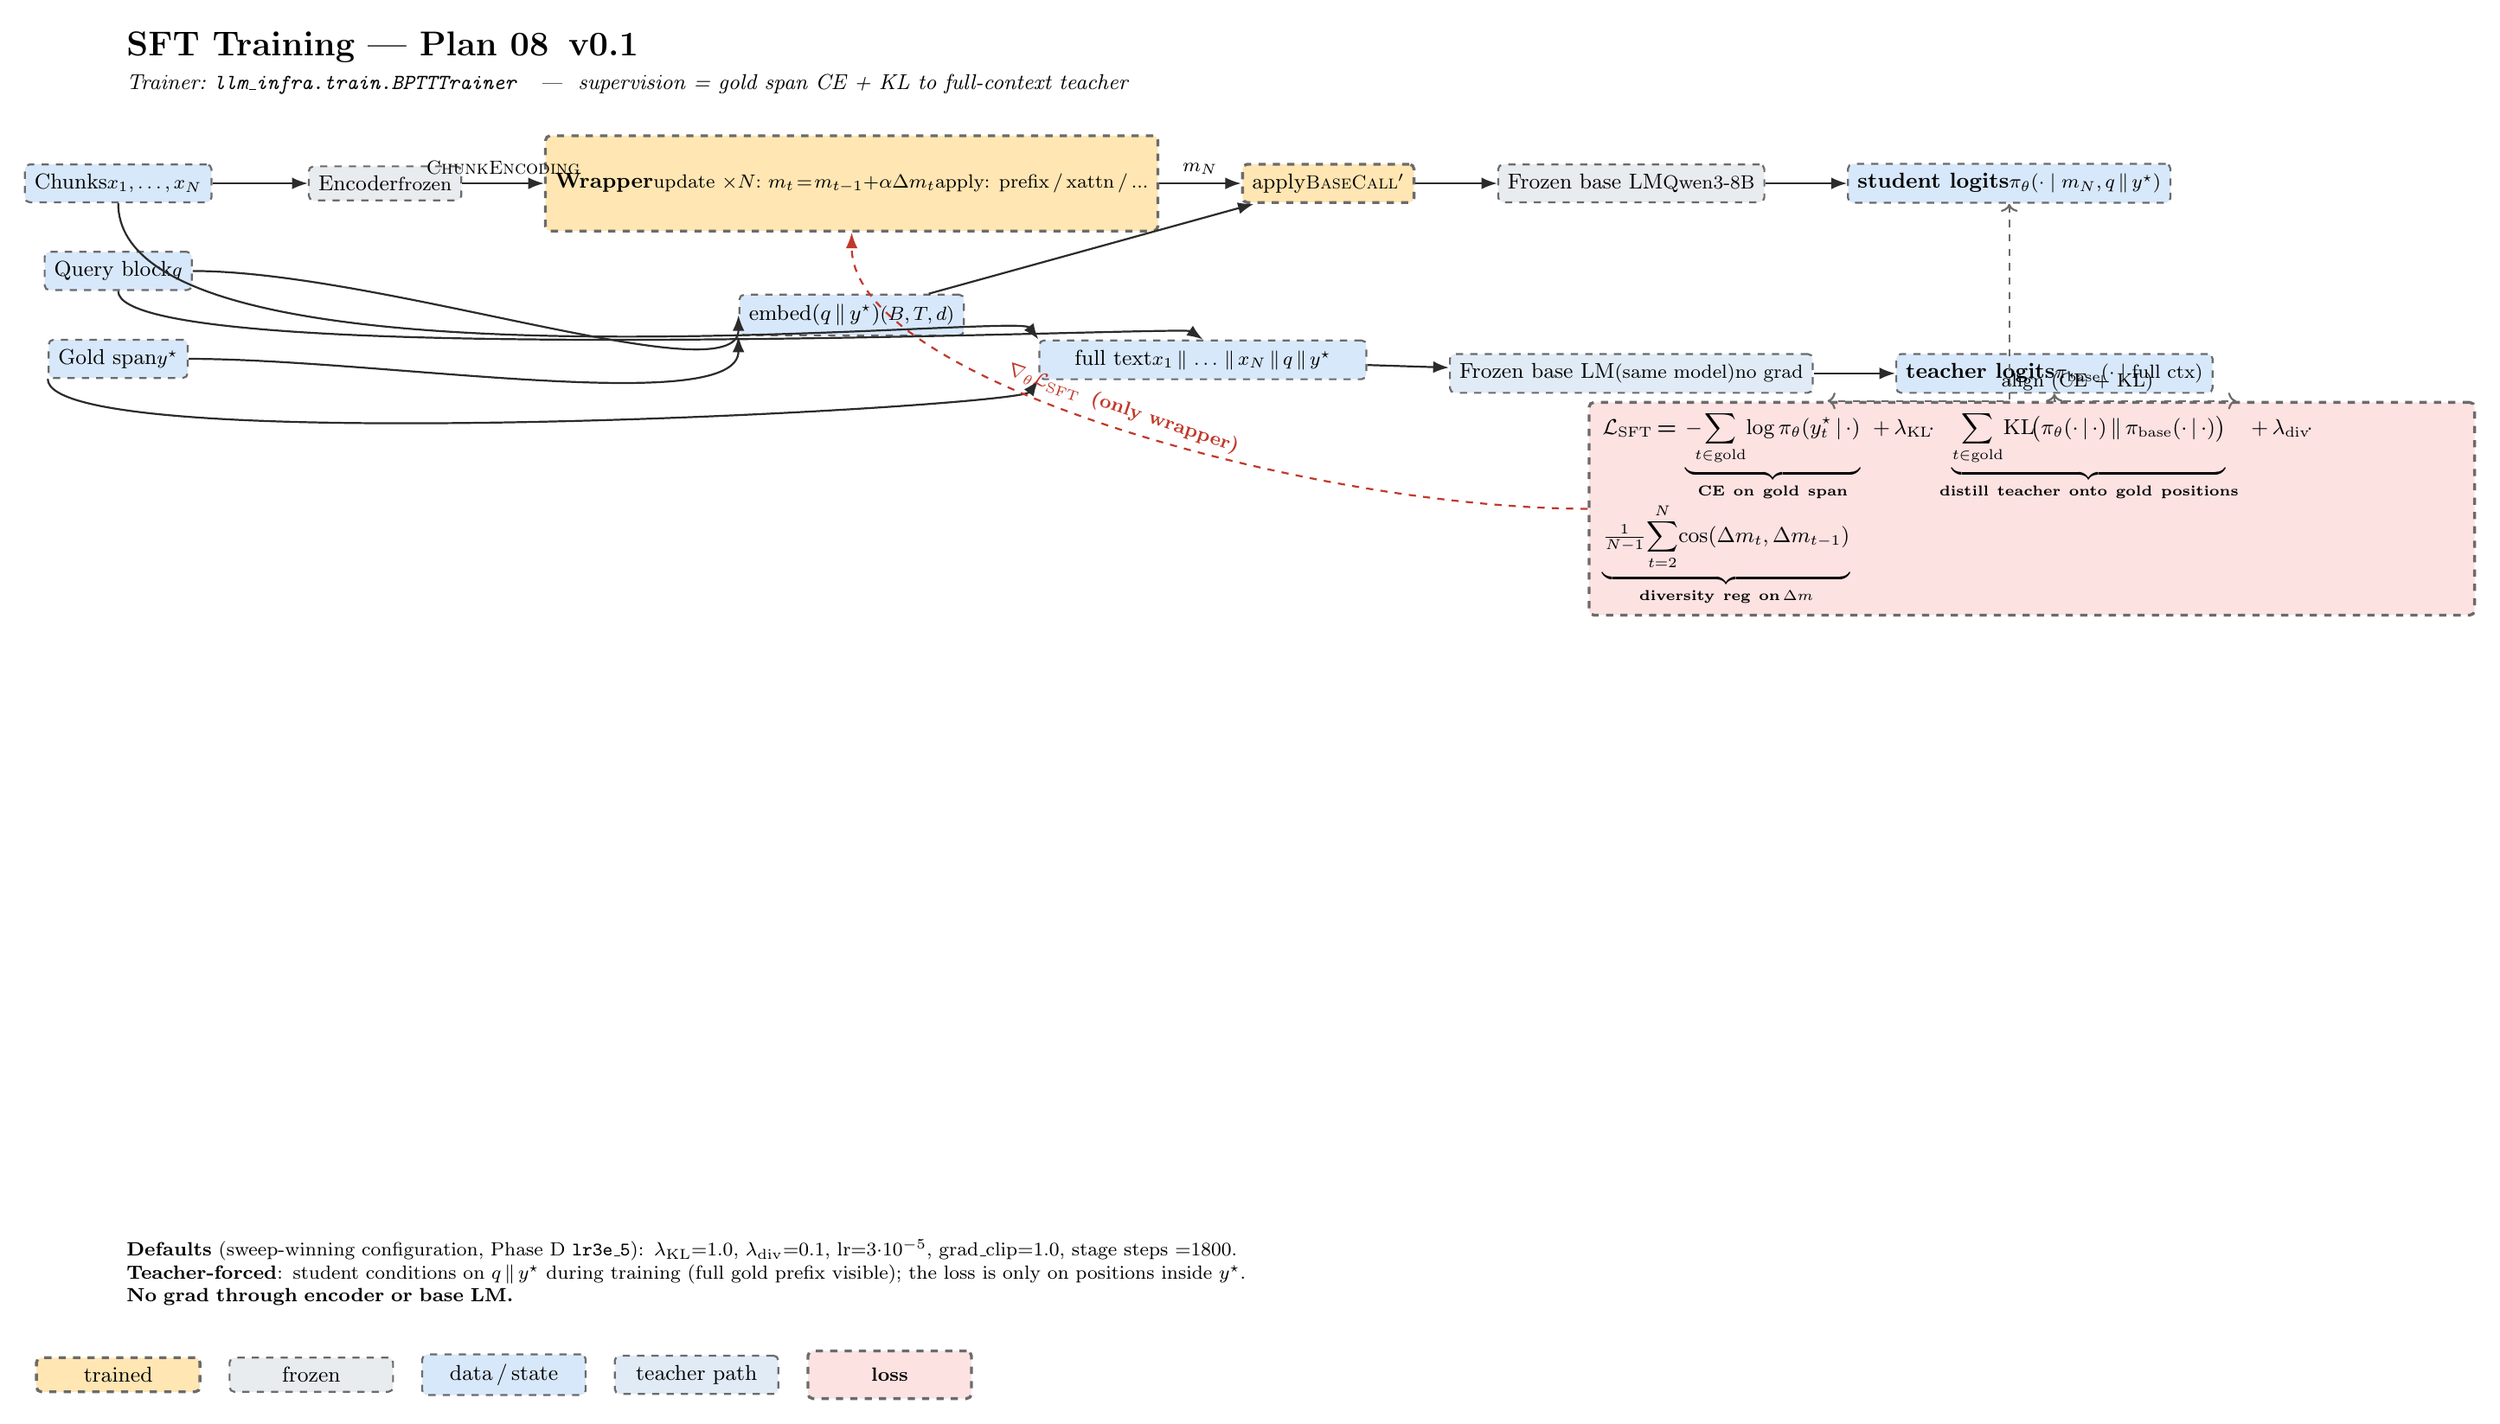
\begin{tikzpicture}[node distance=7mm and 12mm]

%% --- title -------------------------------------------------------------
\node[font=\Large\bfseries, anchor=west] (title) at (0,8.5)
  {SFT Training — Plan 08\ \,v0.1};
\node[font=\small\itshape, anchor=west] at (0,7.95)
  {Trainer:\ \texttt{llm\_infra.train.BPTTTrainer}\ \ \ |\ \
   supervision = gold span CE + KL to full-context teacher};

%% =====================================================================
%% Input data
%% =====================================================================
\node[data]               (chunks) at (0,6.5)
  {Chunks\\\footnotesize $x_1, \dots, x_N$};
\node[data, below=of chunks] (query)
  {Query block\\\footnotesize $q$};
\node[data, below=of query]  (gold)
  {Gold span\\\footnotesize $y^\star$};

%% =====================================================================
%% Student path (with wrapper)
%% =====================================================================
\node[frozen, right=14mm of chunks] (enc_s)
  {Encoder\\\footnotesize frozen};
\node[trained, right=of enc_s, minimum width=44mm, minimum height=14mm] (wrap)
  {\textbf{Wrapper}\\
   \footnotesize update $\times N$:\ $m_t\!=\!m_{t-1}{+}\alpha\Delta m_t$\\
   \footnotesize apply: prefix\,/\,xattn\,/\,...};
\node[data, below=of wrap, yshift=-2mm] (qg_emb)
  {embed$(q\,\|\,y^\star)$\\\footnotesize $(B,T,d)$};
\node[trained, right=of wrap, minimum width=22mm] (apply_s)
  {apply\\\footnotesize\textsc{BaseCall}$'$};
\node[frozen, right=of apply_s, minimum width=28mm] (base_s)
  {Frozen base LM\\\footnotesize Qwen3-8B};
\node[data, right=of base_s] (logits_s)
  {\textbf{student logits}\\\footnotesize $\pi_\theta(\cdot\mid m_N, q\,\|\,y^\star)$};

\draw[flow] (chunks) -- (enc_s);
\draw[flow] (enc_s)  -- node[above,font=\footnotesize]{\textsc{ChunkEncoding}} (wrap);
\draw[flow] (query.east) .. controls +(28mm,0) and +(0,-12mm) .. (qg_emb.west);
\draw[flow] (gold.east)  .. controls +(28mm,0) and +(0,-12mm) .. (qg_emb.south west);
\draw[flow] (qg_emb) -- (apply_s);
\draw[flow] (wrap) -- node[above,font=\footnotesize]{$m_N$} (apply_s);
\draw[flow] (apply_s) -- (base_s);
\draw[flow] (base_s) -- (logits_s);

%% =====================================================================
%% Teacher path (no wrapper, full context, no grad)
%% =====================================================================
\node[teacher, below=22mm of base_s, minimum width=28mm] (base_t)
  {Frozen base LM\\\footnotesize (same model)\\\footnotesize no grad};
\node[data, left=of base_t, yshift=2mm, minimum width=48mm] (cat_t)
  {full text\\\footnotesize $x_1\,\|\,\dots\,\|\,x_N\,\|\,q\,\|\,y^\star$};
\node[data, right=of base_t] (logits_t)
  {\textbf{teacher logits}\\\footnotesize $\pi_{\mathrm{base}}(\cdot\mid \text{full ctx})$};

\draw[flow] (chunks.south)      .. controls +(0,-30mm) and +(-3mm,4mm) .. (cat_t.north west);
\draw[flow] (query.south)       .. controls +(0,-12mm) and +(-3mm,2mm) .. (cat_t.north);
\draw[flow] (gold.south west)   .. controls +(0,-12mm) and +(-3mm,-4mm) .. (cat_t.south west);
\draw[flow] (cat_t) -- (base_t);
\draw[flow] (base_t) -- (logits_t);

%% =====================================================================
%% Loss
%% =====================================================================
\node[loss, below=18mm of $(logits_s)!0.5!(logits_t)$, minimum width=130mm, text width=126mm] (loss)
  {\textbf{$\mathcal{L}_{\mathrm{SFT}}$\,=}\
   $\underbrace{-\!\!\!\sum\limits_{t \in \mathrm{gold}}\!\log \pi_\theta(y^\star_t\,|\,\cdot)}_{\text{CE on gold span}}$
   \,$+\,\lambda_{\mathrm{KL}}\!\cdot\!$
   $\underbrace{\sum\limits_{t \in \mathrm{gold}}\!\mathrm{KL}\!\bigl(\pi_\theta(\cdot\,|\,\cdot)\,\|\,\pi_{\mathrm{base}}(\cdot\,|\,\cdot)\bigr)}_{\text{distill teacher onto gold positions}}$
   \,$+\,\lambda_{\mathrm{div}}\!\cdot\!$
   $\underbrace{\tfrac{1}{N{-}1}\!\sum\limits_{t=2}^{N}\!\cos(\Delta m_t,\Delta m_{t-1})}_{\text{diversity reg on}\,\Delta m}$};

\draw[align] (logits_s) |- ($(loss.north)+(-30mm,0)$)
  node[midway,above,font=\footnotesize,xshift=10mm]{align (CE + KL)};
\draw[align] (logits_t) |- ($(loss.north)+(30mm,0)$);

%% =====================================================================
%% Gradient flow — ONLY to wrapper
%% =====================================================================
\draw[grad] (loss.west) .. controls +(-40mm,0) and +(0,-22mm) .. (wrap.south)
  node[midway,above,font=\footnotesize\bfseries,text=gradclr,sloped]
  {$\nabla_\theta\mathcal{L}_{\mathrm{SFT}}$\ \,(only wrapper)};

%% =====================================================================
%% Notes
%% =====================================================================
\node[font=\footnotesize, anchor=west, text width=170mm] at (0,-9.5)
  {\textbf{Defaults} (sweep-winning configuration, Phase D \texttt{lr3e\_5}):
   $\lambda_{\mathrm{KL}}{=}1.0$,\ $\lambda_{\mathrm{div}}{=}0.1$,\ lr${=}3{\cdot}10^{-5}$,\ grad\_clip${=}1.0$,\
   stage steps ${=}1800$.\ \,
   \textbf{Teacher-forced}: student conditions on
   $q\,\|\,y^\star$ during training (full gold prefix visible);
   the loss is only on positions inside $y^\star$.
   \textbf{No grad through encoder or base LM.}};

%% --- legend ------------------------------------------------------------
\begin{scope}[shift={(0,-11.0)}, font=\footnotesize]
  \node[trained, minimum width=24mm]            (k1) {trained};
  \node[frozen,  right=4mm of k1, minimum width=24mm] (k2) {frozen};
  \node[data,    right=4mm of k2, minimum width=24mm] (k3) {data\,/\,state};
  \node[teacher, right=4mm of k3, minimum width=24mm] (k4) {teacher path};
  \node[loss,    right=4mm of k4, minimum width=24mm,
                 minimum height=7mm, font=\footnotesize\bfseries] (k5) {loss};
\end{scope}

\end{tikzpicture}
\end{document}
